\part{Introduction}

\chapter{Introduction and main objectives}
In human history the presence of disease, caused by parasite is always existed. 
Because of the lack of knowledge about medical science and the poor hygienical conditions the deaths caused by infections in history  have had dramatic repercussion on population life. During the bubonic plague of the 14th century for example 25 million of deaths were reported in Europe out of a population of 100 million. 
During the colonization of the Americas the disease imported by the Europeans is one of the main causes of the genocide of the local population. Diseases like smallpox and cholera were unknown in these countries and native americans have not antibodies to them. 



Not only diseases like these two have am incredible cost in term of human life. They have also effect on historical effect. Due to plague in fact in Europe starts the persecution against Jewish people, considered responsible of the illness spread. While in the Americas, the new infection were one of the element that permits at colonist to subdue the inhabitants. 
Others important epidemic, famous for their consequences were Spanish influenza, Smallpox, Typhus, HIV/AIDS and the more recent Covid-19. 
Because of these, is straightforward evidence of the effect that diseases have on our life.

Only in the last three centuries and just in the most developed countries, like Europe and North America, a significant increase in life expectancy have been observed. The mortality is decreased, but the modification in social patterns and the develop of large cities, have had some consequence. It was increased in the $18^{th}$ and $19^{th}$ centuries the frequency and magnitude of epidemics. 
For this reason diseases are an inevitable agents that is involved in our life. Their implications do not concern only our health status. When we are sick, there are modification in our relationship, work, social life. There is also an economic cost to be healed. Only in few nations worldwide treatment is covered free of charge by the state. In the majority, be ill can result in having to sustain excessive cost. Often due to this, people going into debit or to not take care. 
Nowadays, but also in the past when a new disease appears it is very important try to understand its origin, the biological mechanism under its spread, comprehend its resistance to existent drugs and so on. In practice collect all the information available to understand what is happening.  
These are part of the epidemiological investigation. Other key dimensions are for example genetic resistance, selective pressure of a disease on different human communities, the mechanism underline the acquisition of immunity. Using this knowledge epidemiology try to make a step further of only reconstruct the cause behind the development of a disease: model how can evolute during time. 
\begin{figure}[hbt!]
	\centering
	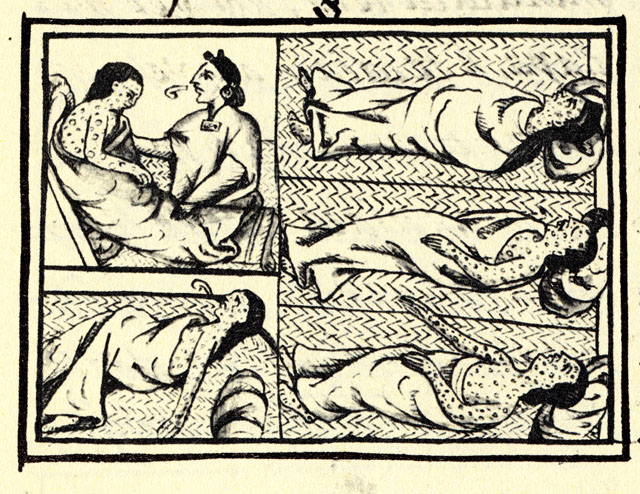
\includegraphics[width=0.4\linewidth]{0_introduction/images_introduction/FlorentineCodex_smallpox}
	\caption[smallpox on native Americans]{Representation of smallpox disease on the Mexican population in the $XIV$ century. Figure from the Florentine Codex \cite{Sahagun1965}. }
	\label{fig:florentinecodexsmallpox}
\end{figure}
There is a lot of interest about this topic both from a scientific perspective and also for public society regulations.
Develop a model that can give us the capability of estimate phenomena like the spread of a disease have a multitude of effects and outcomes on the society.  Social and economic costs are related to every illness, but develop instruments to better understand its impact can avoid the losses of human life and permit to have less serious effect on the society. 
A first simple example, that can help to understand the beneficial effect of study epidemics is the possibility to develop instruments that can permits to consider the specificity of each different disease with "simple" parameters and obtain information like:

\begin{itemize}
	\item is this disease so infective that can cause a pandemic?
	\item what are the threshold conditions that can cause and outbreak? 
\end{itemize}


At a first look the problem can seem simple. Unfortunately, the creation of a model capable of perform an evaluation like the one explained above, suitable for every disease is a problem for which there is not still a solution. 
Every research about the creation of a model that try to represent a real phenomenon must confront with the necessity to simplify, while trying to not loss in accuracy. 
So, in a century of research, many different aspects regarding an epidemic have been considered. The scientist try to catch the most significant ones to develop their model and then figure out if it is capable to give them insights about the considered disease. 
% Qui sarebbe carino iniziare con un discorso che spieghi un po' gli obbiettivi del lavoro 



% ! Ci sta inizialmente concentrarsi sulle epidemie, ma  devi intrudurre anche il secondo macro filone, quello delle opinioni. é uno spin off metodologico del primo, quindi gli stumenti matematici poi sono simili, ma va detta anche questa cosa. E poi sulle opinioni hai visto quante sfumature diverse esistono sul come considerarle e anche questo è da tenere in considerazione. 

\section{Epidemiological theory foundations}

Definition of the theoretical basis and main concepts that will be used in the present work. 
\subsection{ Epidemiologic research historical background}
% Se ti piace l'idea di fare un piccolo excursus storico, va bene. Le info principali sono:
% 1- primo lavoro di Bernoulli
% 2- lavori di Hamer (1906) mass action principle, epidemic description in discrete time 
% 3- Ross, formulation in continous time 
% 4- Kermack and Mc Kendrick (1927) che danno risultato bello perchè introducono "legge" del thresold di una epidemia
% Dopo aver scritto quest'ultimo evento hai il LA per parlare di come funziona un mean field model. 

The research field regarding the development of technique to understand how epidemics can evolve during time has a history starting back in the 20th century. The first important discovery in this field must be attributed to the scientists that find the mechanism used by disease to spread. 
A first innovative work is the one done by John Snow, that during an epidemic of Cholera in London in 1854 successfully determined the source of the infection, even without knowing its etiological agent. Then advancing in the microbiological research is conducted by Pasteur and Koch. They found the etiological agent of disease, enabling the possibility to treat and prevent people from an infection. 
Then, Hamer work in 1906 added a first major theoretical contribution. He formulated a theory about the correlation between the course of an epidemic and the interaction, contact ratio, between susceptible and infectious individuals. It is the so called “mass -action” principle. The number of contacts between these two groups determines the spread rate of the disease. 
This law originally written in discrete time, is then updated in 1908 by Ross, that re-written it  in continuous time. For the first time the problem can be studied using a clearly, well defined mathematical theory. Then the contributions of Kermack and McKendrick in 1927 add another fundamental principle to the modern epidemiology. They formulated a threshold theory explaining which condition can generate the development of an epidemic. The theorem affirms that a certain value must be exceed, depending on the proportion of susceptible and infectious individual. Controlling this value permits to understand if the number of infections will increase, until a peak is reached or if the epidemic is a descendent phase \cite{Mata2021}, \cite{Anderson_82}. 
Their contribution with the mass action principle represents the base for the mean field model theory, that will be presented and analysed in section \ref{subsec:SIR}. 



\subsection{Epidemiological glossary}
To permit a better comprehension of the subject analyzed in the present work a list of principal concepts and terms is presented.

\subsubsection{Micro and Macro parasite}
	The first difference when presenting infection is distinguishing the type of origin that can cause it. An etiological organism responsible for a disease can be divided into microparasite and macroparasite. The former live and reproduce within the host, generating an immune response and the infections caused by them usually have two possible outcomes: death or immunity. Infections origins from them are shorter than the life span of an individual, and so have a transient nature.
\subsubsection{Types of infectious diseases}
Infectious disease is indicated as an illness resulting from the presence of a pathogenic microbial agent. It is possible to distinguish a difference between \textit{transmittable} and \textit{communicable} disease. A transmittable disease can transmitted between persons through unnatural forces. A disease is communicable when the transmission happens directly or indirectly.

\subsubsection{Disease transmission} A disease can transmit in different ways: 
	\begin{itemize}
		\item person to person, for example sexual transmission, involving direct or indirect contact.
		\item airborne, through inhalation of infected air.
		\item food or water borne, ingesting contaminated food. 
		\item vector born, the contagion is caused by infected animals.
	\end{itemize}
	Furthermore when the diffusion is among the same generations is called horizontal transmission, while vertical transmission is the one developing between different generations, from parents to children. 
	Zoonosis is the phenomenon in which a disease that starts in an animal species mutates and attacks humans. The opposite can also happen and it is called inverse-zoonosis. 
	
\subsubsection{Epidemic disease} It occurs when there is a disease with a rapid outbreak, in less than a year there is its development and a peak is reached. The illness is confined to a limited region

\subsubsection{Endemic disease} It is a disease that lasts for a long time and requires consideration of its impact on population renewal and in the number of susceptible individuals.

\subsubsection{Pandemic disease} It is an epidemic that diffuses across multiple regions, on a global scale. The severity of the disease also makes a distinction in calling a disease a pandemic. For example, a common cold is diffused in the whole world but is not defined as a pandemic by the WHO (World Health Organization). 

\subsubsection{Incubation, Symptoms, Infected and Infectious}   A person having contact with another infectious individual, can or not become infected. The incubation is the period after being infected in which the infection increases in size or number in the host but does not produce the symptoms, that are the effect of the disease. 

\subsubsection{Outbreak} Is the rapid raise in the number of infected during an epidemic.

\subsubsection{Incidence and prevalence} The first term refers to the number of new cases after a certain period (daily or weekly for example), while prevalence is the proportion of the population affected by a disease in a specific time.

\subsubsection{Immunity and herd immunity} Immunity is protection from a disease gained after having contracted it. It can last forever or vanish after a certain time. New exposure to the virus does not lead to infection. Herd immunity is instead an important phenomenon in which the defense against a disease is due to the majority of the population being immune, thanks to vaccines or surviving it. This majority protects the rest of the population because slows down the diffusion or stops the spread of the illness.

\subsubsection{Virulence and Contagiousness}  Virulence is used to describe how aggressive, harmful, and pathogenic is a biological agent in attacking cells. Contagiousness is referred to an individual and it is used to represent the capability to transmit a disease. 

\subsubsection{Overdispersion and Superspreading} Overdispersion is a term that refers to observing a larger variance than expected from a normal distribution. It is used in statistics to measure superspreading, a circumstance in which there is an anomaly (higher) number of secondary infections.

\subsubsection{CFR, IFR and mortality excess} The case fatality rate is the ratio between the number of deaths due to a specific disease and the total number of confirmed positive cases. It is the likelihood for an infected person to die because of the infection. The infection fatality rate is instead the percentage of people infected with the disease that are expected to die. The two quantities can have a similar value: if every person who contracts the disease and every death attributable to the disease is known and recorded, then the CFR will equal the IFR.
The excess in mortality can be calculated by observing the difference between the total death rate (due to any reason) a month per month in a comparison between a year with an epidemic and one without. 

\subsubsection{Reproduction number $R_0$}

\subsubsection{Incubation period and serial interval} The incubation is the time after exposure in which the disease develop and end when the infect starts show symptoms. 

%%%%%%%%%%%%%%%%%%%%
\section{Epidemiological models categorization }
There are several different typologies of mathematical model developed to describe the course of an epidemic. In this section the principal categories are introduced. There is then a focus, in \ref{subsec:SIR}, on the one used for the development of the present work, useful to introduce its main mechanisms and the first important conclusion that can be derived from it. 

\subsection{Mean field models}

The mean field model, also known as compartmental models are the first and most studied typology of mathematical model used in epidemiology.  The population considered in the model is divided in several subgroups, on the basis of the dynamic that want to be described. In this class of model  the severity of infection usually is not considered. People are infected or not. The transition from one compartment to another is determined by differential equations. There are transmission rates from one class to another. 

\subsubsection{SIR model}

\subsection{Stochastic models}
In this typology of models, the transition from a state to another is determined using a function of probability. They can be conceptually derived starting from the framework represented by ODEs models. They are useful when the disease to study has a lower number of infected or if there is a connection between the epidemic outcome and changes in individual dynamics. This is called demographic variability, and it concerns changes in transmission, births, recovery, or deaths within the population. Using stochastic models with Monte Carlo simulations can be useful to investigate epidemic models on networks. 
The two most important type of models using this approach consider the time variable as continuous, $t \in [0, \infty) $and then the state variable is either discrete (Continuous-Time Markov-Chain) or continuous (Stochastic Differential Equations).
Referring to the SIR model to make a simple example here the S and I compartments are modelled as random variables. The probability to individuals to change group depends on infection and recovery, the possible events that can occur. It is called transition probability. 
In a Markov chain approach the transition probability is discretised, and there is no dependence on the history of the epidemic to know how it will evolve at time $t + \Delta t$. It is necessary to know only the current state of the process at time $t$. 
In the Stochastic differential equation, the random variables are continuous. The system of equation deriving from this method are usually simpler to solve that the ones find using the first approach\cite{Allen2017}.  

\subsection{Agent-based networks}
Another representation of the disease evolution can be done using an agent-based model. Here, using the topology of a network, composed by nodes and edges is realised the simulation. Individuals are represented with the node and their interactions with the edges. So, the connections in the graph are responsible for the contagion. Using this framework, it is possible to simulate more realistic scenarios, because permits to represent large and heterogeneous systems. It is not easy however to understand how model a complex society in this way.  

\subsection{Multilayer systems}

The complex dynamic of interactions existing in real word, develops in multiple patterns, with complicated relationships. This connection can change in time, and using the theory of multilayer network it can be improved the comprehension of such complexity. This is a more recent development of the research, the traditional network theory was revisited, to create a framework that can include multiple networks, that evolve and influence each other \cite{DeDomenico2016}. 
One possible way to develop models with this structure is the one done imagining that each layer represent a different type of interaction. An epidemiological example is one layer in which the physical contact between people are simulated and another representing social structure, the network of relations that every person has. This case has been presented in multiple works in the last year, for example CITA. 
The dynamic realized in multiple networks can be single or coupled. In the first there is a top layer with its own dynamic evolution influencing another one. The coupled structure instead is the one in which the phenomena described in each layer evolve with the influence of what is happening in the other. There is a coupled connection with the presence of intra-layer connections.




